\documentclass[11pt,aspectratio=169]{beamer}
\newcommand{\TalkShort}{Satellite cloud data over France}
% Visual reference: Matteo Di Sante, 13_06_26_slides_soaring_ctrw.tex.
% Steel-blue title bar, Palatino, Pisa seal, white pages and a pale title band.
\usepackage[T1]{fontenc}
\usepackage[utf8]{inputenc}
\usepackage[english]{babel}
\usepackage{mathpazo}
\usefonttheme{serif}
\usepackage{amsmath,amssymb,bm,booktabs,array,graphicx,tikz,microtype}
\usetikzlibrary{arrows.meta,calc,positioning}
\usepackage{siunitx}
\sisetup{group-separator={,},group-minimum-digits=4}
\usepackage{pgfpages}
\ifdefined\Speakernotes
  \setbeameroption{show notes on second screen=right}
\else
  \setbeameroption{hide notes}
\fi
\definecolor{pisablue}{RGB}{74,96,121}
\definecolor{pisablight}{RGB}{192,206,220}
\definecolor{accent}{RGB}{26,118,179}
\definecolor{para}{HTML}{3477A8}
\definecolor{hang}{HTML}{B5482A}
\definecolor{beginner}{HTML}{6A3D9A}
\definecolor{expert}{HTML}{C98A1E}
\definecolor{teal}{HTML}{2E7D8A}
\definecolor{wine}{HTML}{8E3B5C}
\definecolor{muted}{HTML}{666666}
\setbeamercolor{structure}{fg=pisablue}
\setbeamercolor{normal text}{fg=black,bg=white}
\setbeamercolor{frametitle}{fg=white,bg=pisablue}
\setbeamercolor{alerted text}{fg=accent}
\setbeamercolor{block title}{fg=white,bg=pisablue}
\setbeamercolor{block body}{fg=black,bg=pisablight!28}
\setbeamercolor{discussion}{fg=pisablue,bg=pisablight!30}
\setbeamercolor{button}{fg=white,bg=pisablue}
\setbeamerfont{button}{size=\normalsize}
\setbeamersize{text margin left=7mm,text margin right=7mm}
\setbeamertemplate{navigation symbols}{}
\setbeamertemplate{itemize item}{\textcolor{pisablue}{\small$\bullet$}}
\setbeamertemplate{itemize subitem}{\textcolor{pisablue}{\textendash}}
\setbeamertemplate{itemize/enumerate body begin}{\setlength{\itemsep}{0.55em}}
\setbeamertemplate{frametitle}{%
  \nointerlineskip
  \begin{beamercolorbox}[wd=\paperwidth,ht=9mm,dp=3mm,center]{frametitle}
    \large\insertframetitle\strut
  \end{beamercolorbox}
  \begin{tikzpicture}[remember picture,overlay]
    \node[anchor=north east,text=white,inner sep=0pt,xshift=-2.3mm,yshift=-4.2mm]
      at(current page.north east){\small\insertframenumber};
  \end{tikzpicture}
}
\setbeamertemplate{footline}{%
  \hspace{7mm}\textcolor{muted}{\fontsize{6.5}{8}\selectfont
    Matteo Di Sante\enspace|\enspace\TalkShort}\vspace{2mm}
}
\newcommand{\kw}[1]{\textcolor{accent}{#1}}
\newcommand{\source}[1]{\par\vspace{1mm}{\fontsize{7}{8.3}\selectfont\color{muted}#1\par}}
% Discussion prompts belong only on the companion notes page.
\newcommand{\question}[1]{\note{\par\textbf{Discussion.} #1\par\medskip}}
\newcommand{\takeaway}[1]{\par\vfill
  \begin{beamercolorbox}[wd=\linewidth,sep=5pt]{discussion}
    \small #1
  \end{beamercolorbox}}
\newcommand{\fig}[2][54mm]{\includegraphics[width=\linewidth,height=#1,keepaspectratio]{assets/#2}\par}
\newcommand{\speaker}[1]{\note{#1}}
\setbeamertemplate{note page}{%
  \vspace{4mm}\noindent%
  \begin{minipage}{\linewidth}
    {\small\color{pisablue}\TalkShort\quad|\quad Slide \insertframenumber}\par\medskip
    {\normalsize\bfseries\insertframetitle}\par\medskip
    {\small\insertnote}
  \end{minipage}
}
\newcommand{\refitem}[3]{\href{#1}{#2}\hfill {\color{muted}#3}\par\medskip}
\newcommand{\titleframe}[4]{%
\begin{frame}[plain]
\begin{tikzpicture}[remember picture,overlay]
 \fill[pisablue](current page.south west)rectangle(current page.north east);
 \fill[pisablight](current page.south west)rectangle([yshift=20mm]current page.south east);
 \node[text=white,align=center,text width=.92\paperwidth]at(current page.center)
   {{\LARGE\bfseries #1}};
 \node[text=pisablue,align=center]at([yshift=10mm]current page.south)
   {{\normalsize Version: 14/09/2026}\\[2mm]
    {\small #3}};
\end{tikzpicture}
\note{#4}
\end{frame}}
% Marks a thesis subsection boundary: a PDF bookmark plus a full-page divider,
% so each block of slides can be traced back to its exact place in the thesis.
\newcommand{\subsectionframe}[2]{%
\subsection{#2}
\begin{frame}[plain,noframenumbering]
\begin{tikzpicture}[remember picture,overlay]
 \fill[pisablue](current page.south west)rectangle(current page.north east);
 \node[text=pisablight,align=center,text width=.82\paperwidth]
   at([yshift=10mm]current page.center){{\normalsize Thesis~\S#1}};
 \node[text=white,align=center,text width=.82\paperwidth]
   at([yshift=-4mm]current page.center){{\Large\bfseries #2}};
\end{tikzpicture}
\end{frame}}
\newcommand{\backupstart}{%
\appendix
\begin{frame}[plain,noframenumbering]
\begin{tikzpicture}[remember picture,overlay]
 \fill[pisablue](current page.south west)rectangle(current page.north east);
 \node[text=white,align=center]at(current page.center)
  {{\LARGE\bfseries Discussion material}\\[4mm]{\large Extra figures, derivations and references}};
\end{tikzpicture}
\end{frame}}
\hypersetup{colorlinks=true,urlcolor=accent,linkcolor=accent,pdfauthor={Matteo Di Sante}}
% A notes sheet contains a second rendering of the slide. Disable its duplicate
% destinations; the normal slide PDF retains all hyperlinks and the viewer button.
\ifdefined\Speakernotes\hypersetup{draft}\fi

\usepackage{tabularx}
\usepackage{textcomp}
\usepackage{animate}
\hypersetup{pdftitle={Satellite cloud data over France},pdfsubject={Data survey for the Thermal-planes cells}}
\definecolor{sevfull}{HTML}{8FB0C9}
\definecolor{sevrss}{HTML}{2F6690}
\definecolor{mtg}{HTML}{C2610F}
\definecolor{mtglight}{HTML}{E8913A}
\definecolor{gap}{HTML}{E8C9A6}
\definecolor{feasible}{HTML}{9C4A06}
\newcommand{\faint}[1]{{\small\color{muted}#1}}
\newcommand{\stepitem}[2]{\noindent\makebox[6mm][l]{\textcolor{pisablue}{\bfseries #1}}\parbox[t]{\dimexpr\linewidth-6mm}{\raggedright #2}\par}
\newcommand{\bignum}[2]{{\color{#1}\LARGE\bfseries #2}}
\newcolumntype{L}{>{\raggedright\arraybackslash}X}
\newcolumntype{P}[1]{>{\raggedright\arraybackslash}p{#1}}
\title{Satellite cloud data over France}
\begin{document}

\begin{frame}[plain]
\begin{tikzpicture}[remember picture,overlay]
 \fill[pisablue](current page.south west)rectangle(current page.north east);
 \fill[pisablight](current page.south west)rectangle([yshift=20mm]current page.south east);
 \node[inner sep=0pt]at([yshift=20mm]current page.center)
  {
\includegraphics[width=52mm]{assets/satellite-cover.png}};
 \node[text=white,align=center,text width=.9\paperwidth]at([yshift=-7mm]current page.center)
  {{\LARGE\bfseries Satellite cloud data over France}};
 \node[text=pisablue,align=center]at([yshift=10mm]current page.south)
  {{\normalsize Matteo Di Sante}\\[1mm]{\small Data survey, 7 October 2026}};
\end{tikzpicture}
\speaker{First an overview of the satellite cloud data available over France: which satellites, which years, how sharp, which products, and their limits. Then what our study of the twelve Thermal-planes cells needs, and how much space that takes.}
\end{frame}

\section{Overview}

\begin{frame}{Two kinds of satellites}
\vspace{1mm}
{\small\renewcommand{\arraystretch}{1.3}
\begin{tabularx}{\linewidth}{@{}P{28mm}P{38mm}P{24mm}L@{}}\toprule
\textbf{Orbit} & \textbf{Images of the same area} & \textbf{Pixel size} & \textbf{Examples}\\\midrule
\textcolor{mtg}{\textbf{Geostationary}} & Every 2.5--15\,min\textsuperscript{*} & 0.6--5\,km & MSG (SEVIRI), MTG (FCI)\\[1mm]
\textcolor{sevrss}{\textbf{Polar orbiting}} & 1--2 per day, or every few days for finer images & 10\,m--1\,km & Sentinel-2, Landsat, MODIS, VIIRS\\\bottomrule
\end{tabularx}}
\vspace{2mm}
\begin{columns}[c,onlytextwidth]
\column{.53\textwidth}
{\textcolor{mtg}{\textbf{Geostationary}}}\par\smallskip
\textbf{Keeps the same region in view.}\par\medskip
{\textcolor{sevrss}{\textbf{Polar orbiting}}}\par\smallskip
Passes near the poles.\par
\textbf{Sees a new strip as Earth turns.}
\column{.43\textwidth}\centering
\ifdefined\Speakernotes
 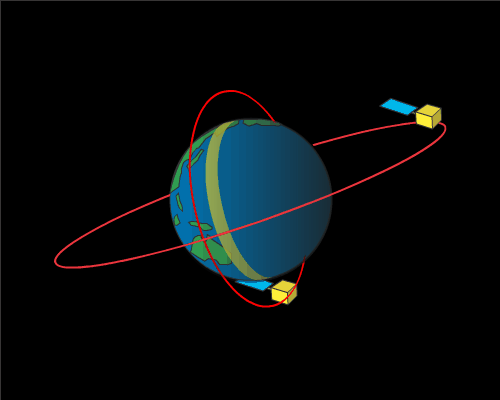
\includegraphics[height=28mm]{assets/orbits/frames/frame-18.png}
\else
 \animategraphics[autoplay,loop,poster=18,height=28mm]{10}{assets/orbits/frames/frame-}{00}{71}
\fi\par
{\footnotesize\href{run:assets/orbits/orbits.gif}{Open GIF}}
\end{columns}
\source{\textsuperscript{*}2.5\,min: planned MTG rapid scan. Animation: \href{https://spaceplace.nasa.gov/orbits/en/}{NASA Space Place}.}
\speaker{Geostationary: Meteosat SEVIRI and MTG FCI, fixed above the equator relative to the rotating Earth, imaging Europe every few minutes. The 2.5-minute cadence refers to the planned MTG-I2 rapid scan, not the current service. Polar orbiting satellites pass at 700--800 km. Revisit depends on the instrument and swath: MODIS and VIIRS provide about one or two daytime views per day, while the finest images are less frequent. Sentinel-2 (10--60 m, every 2--5 days, about 10:30), Landsat 8 and 9 (30 m, every 8 days), MODIS (250 m--1 km, about 10:30 and 13:30), VIIRS (375 m, about 13:30). Geostationary images follow clouds through the day; polar images can resolve individual cumuli for validation. Animation credit: NASA Space Place, What Is an Orbit?, https://spaceplace.nasa.gov/orbits/en/, original GIF geostationary-and-polar-orbits.en.gif. It shows equatorial and near-polar motion while Earth turns; distances, spacecraft sizes and relative speeds are schematic. Orbital interpretation checked against ESA, Types of orbits, https://www.esa.int/Enabling\_Support/Space\_Transportation/Types\_of\_orbits. Other SEVIRI-based options: CM SAF CLAAS-3, a climate-quality cloud record every 15 minutes from 2004; the NWC SAF software of Meteo-France, which needs the full image files.}
\end{frame}

\begin{frame}{Full disc or rapid scan: the whole view or only Europe}
\vfill
\begin{columns}[c,onlytextwidth]
\column{.36\textwidth}\centering
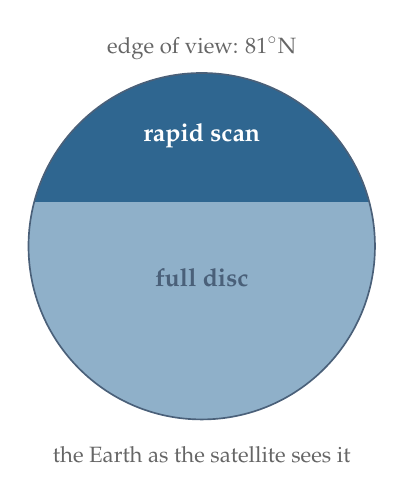
\begin{tikzpicture}
 \fill[sevfull](0,0)circle(2.2);
 \begin{scope}\clip(0,0)circle(2.2);\fill[sevrss](-2.3,0.56)rectangle(2.3,2.3);\end{scope}
 \draw[pisablue,line width=.6pt](0,0)circle(2.2);
 \node[anchor=south,font=\footnotesize,text=muted]at(0,2.25){edge of view: 81$^\circ$N};
 \node[text=white,font=\small\bfseries]at(0,1.4){rapid scan};
 \node[text=pisablue,font=\small\bfseries]at(0,-.4){full disc};
 \node[font=\footnotesize,text=muted]at(0,-2.65){the Earth as the satellite sees it};
\end{tikzpicture}
\column{.6\textwidth}
{\large\textcolor{sevfull!70!black}{\textbf{Full disc}}}\par\smallskip
All the Earth the satellite sees, about 40\% of the globe\par\bigskip
{\large\textcolor{sevrss}{\textbf{Rapid scan}}}\par\smallskip
Only the northern third: Europe and North Africa.\par
Smaller area, scanned more often: with SEVIRI (MSG) every 5\,min instead of 15.
\end{columns}
\vfill
\takeaway{France is in both}
\speaker{SEVIRI full disc: every 15 minutes, from the prime Meteosat above 0 degrees. SEVIRI rapid scan: the top third of the disc, about 15 to 70 degrees north, every 5 minutes, from a second Meteosat rectified to 9.5 degrees east (EUMETSAT product description). MTG: full disc every 10 minutes; its rapid scan, every 2.5 minutes, comes with MTG-I2. A geostationary satellite never sees the whole world, only the hemisphere facing it. The rapid scan has service gaps that the full disc can fill at 15 minutes.}
\end{frame}

\begin{frame}{Which geostationary satellite covers which years}
\vfill\centering
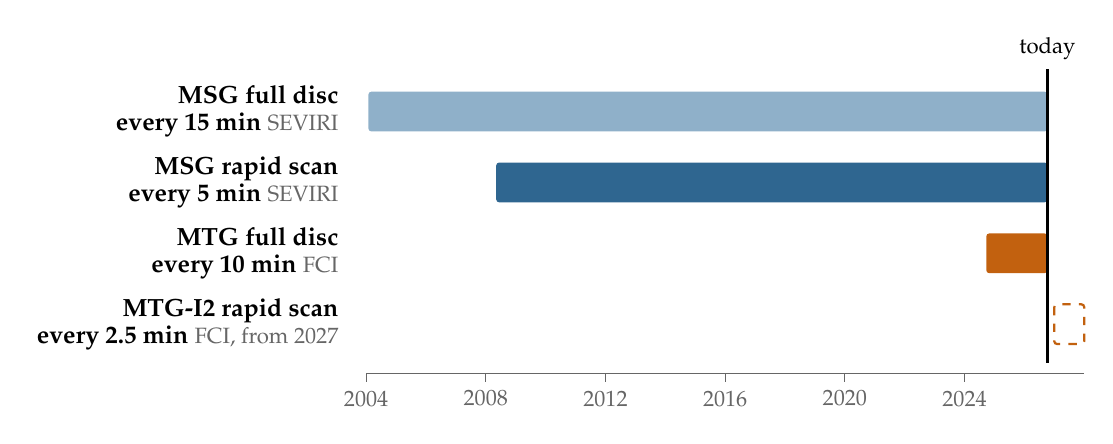
\begin{tikzpicture}[x=3.8mm,y=-9mm,font=\small]
 \foreach \row/\name/\detail in {0/MSG full disc/{\textbf{every 15 min} {\color{muted}\footnotesize SEVIRI}},1/MSG rapid scan/{\textbf{every 5 min} {\color{muted}\footnotesize SEVIRI}},2/MTG full disc/{\textbf{every 10 min} {\color{muted}\footnotesize FCI}},3/MTG-I2 rapid scan/{\textbf{every 2.5 min} {\color{muted}\footnotesize FCI, from 2027}}}{
  \node[anchor=east,align=right]at(-0.6,\row){\textbf{\name}\\[-.5mm]{\small\detail}};}
 \fill[sevfull,rounded corners=1pt](0.08,-0.28)rectangle(22.77,0.28);
 \fill[sevrss,rounded corners=1pt](4.35,0.72)rectangle(22.77,1.28);
 \fill[mtg,rounded corners=1pt](20.73,1.72)rectangle(22.77,2.28);
 \draw[mtg,dashed,line width=.8pt,rounded corners=1pt](23,2.72)rectangle(24,3.28);
 \draw[line width=.8pt](22.77,-0.6)--(22.77,3.55);
 \node[above,font=\footnotesize]at(22.77,-0.6){today};
 \draw[muted](0,3.7)--(24,3.7);
 \foreach \y in {2004,2008,...,2024}{\draw[muted](\y-2004,3.7)--++(0,.12);
  \node[below,font=\footnotesize,text=muted]at(\y-2004,3.8){\y};}
\end{tikzpicture}
\vfill
\takeaway{Full disc is always the slower one: 15 against 5\,min (MSG), 10 against 2.5 (MTG)}
\speaker{Within each generation the full disc is the slower one, because it covers the whole visible Earth while the rapid scan covers only the top third. MSG is Meteosat Second Generation (Meteosat-8 to 11), carrying the imager SEVIRI; MTG is Meteosat Third Generation, carrying the imager FCI. Start dates are the first products in the EUMETSAT Data Store: MSG full disc January 2004, MSG rapid scan May 2008, MTG full disc (Meteosat-12) September 2024, operational since 4 December 2024. MTG-I2 launched on 27 August 2026; its 2.5-minute rapid scan starts after commissioning, in 2027.}
\end{frame}

\begin{frame}{Three kinds of channels, three questions}
\vfill
\renewcommand{\arraystretch}{1.25}
\begin{tabularx}{\linewidth}{@{}P{38mm}Lr@{}}
\multicolumn{2}{@{}l}{\faint{The 12 SEVIRI channels (MTG has 16)}} & \makebox[0pt][r]{\faint{pixel at 45\,$^\circ$N, east--west\,$\times$\,north--south}}\\
{\large\textcolor{sevrss}{\textbf{Visible}}}\newline\faint{daytime} & {\large Where are the clouds?}\newline\faint{VIS0.6 0.56--0.71\,\textmu m, VIS0.8 0.74--0.88\,\textmu m} & {\large 3.2\,$\times$\,5.2\,km}\\
{\large\textcolor{sevrss}{\textbf{Visible, HRV}}}\newline\faint{daytime} & {\large\textbf{The same, with pixels 3 times finer}}\newline\faint{broadband 0.4--1.1\,\textmu m, about 5 times wider than VIS0.6} & {\large\bfseries\textcolor{sevrss}{1.1\,$\times$\,1.7\,km}}\\
{\large\textcolor{feasible}{\textbf{Near-infrared}}}\newline\faint{daytime} & {\large Ice or water?}\newline\faint{NIR1.6 1.50--1.78\,\textmu m} & {\large 3.2\,$\times$\,5.2\,km}\\
{\large\textcolor{mtg}{\textbf{Thermal infrared}}}\newline\faint{day and night} & {\large How cold, so how high?}\newline\faint{8 channels, 3.5--14.4\,\textmu m: IR3.9, WV6.2, WV7.3,}\newline\faint{IR8.7, IR9.7, IR10.8, IR12.0, IR13.4} & {\large 3.2\,$\times$\,5.2\,km}\\
\end{tabularx}
\vfill
\takeaway{HRV: pixels 3 times finer in both directions, and a visible band 5 times wider.}
\speaker{SEVIRI channels, with the lower and upper limit of each spectral band in micrometres (Schmetz et al. 2002, Table 1). Visible: HRV (broadband, about 0.4--1.1, 1 km sampling, against 3 km for the other 11 channels: over France about $1\times2$ against $3\times5$\,km; its band is about 0.7 micrometres wide, 5 times VIS0.6, so it collects more light), VIS0.6 (0.56--0.71) and VIS0.8 (0.74--0.88, at the edge of the near-infrared). Near-infrared: NIR1.6 (1.50--1.78). Thermal infrared, day and night: IR3.9 (3.48--4.36), WV6.2 (5.35--7.15), WV7.3 (6.85--7.85), IR8.7 (8.30--9.10), IR9.7 (9.38--9.94), IR10.8 (9.80--11.80), IR12.0 (11.00--13.00), IR13.4 (12.40--14.40). All 12 come from the same scan, in the same file. Pixel sizes are sampling distances: 3 km and 1 km at the sub-satellite point (equator, 9.5 E for the rapid scan), where the pixel is square. Away from it the pixel stretches, mostly north--south: at 45 N it is 3.2 by 5.2 km and 1.1 by 1.7 km (east--west by north--south); over our cells it ranges from 3.2 by 4.9 km (Pyrenees, 43 N) to 3.3 by 5.9 km (Normandy, 49 N), and HRV is always 3 times finer in both directions. Each pixel sees a little more than its spacing: the field of view is 4.8 km for the 11 channels and 1.67 km for HRV at the sub-satellite point (Schmetz et al. 2002), so neighbouring pixels overlap. MTG FCI: VIS0.4, 0.5, 0.6, 0.8, 0.9, NIR1.3, 1.6, 2.2, and eight infrared channels, on a 1 or 2 km grid; VIS0.6, NIR2.2, IR3.8 and IR10.5 also at 0.5 or 1 km.}
\end{frame}

\begin{frame}{What one pixel holds at one time}
\vfill
{\large 12 channels, each providing its own measurement.}\par
\vspace{9mm}
\begin{columns}[T,onlytextwidth]
\column{.47\textwidth}
{\large\textcolor{sevrss}{\textbf{Reflectance (\%)}}}\par\smallskip
{\small\color{muted}Visible and near-infrared}\par\medskip
How much sunlight is reflected
\column{.49\textwidth}
{\large\textcolor{mtg}{\textbf{Brightness temperature (K)}}}\par\smallskip
{\small\color{muted}Thermal infrared}\par\medskip
How warm or cold it appears
\end{columns}
\vfill
{\small\color{muted}No correction for the Sun's angle: low Sun makes the same ground look darker.}\par
\vspace{3mm}
\speaker{\textbf{Calibration.} SEVIRI's 10-bit counts (0--1023) become radiance through $L=\mathrm{gain}\times\mathrm{count}+\mathrm{offset}$. Solar channels give $R=100\pi L/F$ in percent, with band irradiance $F$ adjusted for Sun--Earth distance. Thermal channels give the equivalent black-body temperature.\par\smallskip
\textbf{Illumination.} The stored reflectance has no solar-zenith correction. For a diffuse surface, $R$ varies with albedo times $\cos(\mathrm{SZA})$: unchanged ground can look darker under a low Sun. Normalising illumination helps distinguish this effect from changes in clouds.\par\smallskip
\textbf{Storage.} Open Climate Fix rescales these quantities to 0--1 using fixed bounds and 16-bit floats. Out-of-range values are clipped, for example HRV above about 104\% or IR10.8 below 199\,K.\par\smallskip
\textbf{Coordinates and time.} $(x,y)$ is the pixel centre, with 3\,km spacing, or 1\,km for HRV, at the sub-satellite point. The image time labels the end of a 5-minute slot. France is scanned about 1.5--2 minutes earlier, estimated from scan geometry. The copy drops original line times; a 17\,km window is scanned within about one second.\par\smallskip
\textbf{Sources.} satpy readers/core/seviri.py and SunZenithCorrector; Open Climate Fix satellite-consumer, process.py; 2020 Zarr store attributes.
}
\end{frame}

\section{The datasets}

\begin{frame}{What can be downloaded}
\vfill
\large\renewcommand{\arraystretch}{1.16}
\begin{tabularx}{\linewidth}{@{}Lrrr@{}}\toprule
 & Every & Years & Whole archive\\\midrule
\multicolumn{4}{@{}l}{\textcolor{sevrss}{\normalsize\bfseries "Images": what the instrument measures}}\\
MSG rapid scan & 5\,min & May 2008 $\to$ & 101\,TB\\
MSG, copy by Open Climate Fix & 5\,min & 2008--2022 & 62\,TB\\
MTG full disc & 10\,min & Sep 2024 $\to$ & 107\,TB\\[1mm]
\multicolumn{4}{@{}l}{\textcolor{feasible}{\normalsize\bfseries Products: one answer per pixel, by EUMETSAT}}\\
MSG cloud mask & 5\,min & Oct 2008 $\to$ & 0.15\,TB\\
MSG cloud-top height & 15\,min & Jun 2005 $\to$ & 0.24\,TB\\
MTG cloud mask & 10\,min & Jan 2025 $\to$ & 0.45\,TB\\
MTG cloud-top height, cloud type & 10\,min & Dec 2025 $\to$ & 3.9\,TB\\\bottomrule
\end{tabularx}
\vfill
\source{Start dates: first product in the EUMETSAT Data Store, checked 6 Oct 2026. MTG images start in Sep 2024, pre-operational; operational since 4 Dec 2024.}
\speaker{All free with a EUMETSAT account; the Open Climate Fix copy needs none. MTG data are public from 24 September 2024, pre-operational until 4 December 2024. Sizes are product counts times mean file size; $\to$ means up to today. Per year the two SEVIRI archives are similar: about 5.5 TB from EUMETSAT and 4.4 TB in the Open Climate Fix copy, which is 25 percent smaller thanks to 16-bit values compressed with zstd; 62 TB is our estimate from the measured 2020 store, close to the 60 TB Open Climate Fix states. SEVIRI images: 58 MB every 5 minutes, all of Europe in one file; a recalibrated record (FCDR, 2008--2021, 102 TB) also exists. MTG images: the 4 high-resolution channels (107 TB) and all 16 channels (105 TB), about 1 GB every 10 minutes each, in 40 horizontal strips of which a French region needs 3. SEVIRI full-disc cloud mask: every 15 minutes since 2004, 0.45 TB. MTG cloud mask since January 2025; cloud-top height and cloud type since December 2025. The rapid scan misses about 7 percent of summer daytime images (70 percent present in 2008, 84--93 percent in 2009--2012, 2017 and 2022, 97--100 percent otherwise); the official archive has the same gaps.}
\end{frame}

\begin{frame}{Two ways to get the same SEVIRI images}
\vfill
{\large\renewcommand{\arraystretch}{1.45}
\begin{tabularx}{\linewidth}{@{}P{38mm}LL@{}}\toprule
 & \textbf{EUMETSAT} & \textbf{Open Climate Fix}\\\midrule
Archive 2008--2022 & $\approx$\,81\,TB & $\approx$\,62\,TB\\[2mm]
One download & \textbf{58\,MB}\newline Whole Europe, one scan & $\approx$\,\textbf{1.4\,MB}\newline Regional block, one hour\\[2mm]
France, one day & $\approx$\,\textbf{8.4\,GB} & $\approx$\,\textbf{0.24\,GB}\\\bottomrule
\end{tabularx}}
\vfill
\takeaway{Open Climate Fix lets us download only the blocks covering France: about 1/35 of the download volume.}
\source{Mainland France, 25 July 2020, 08:00--20:00 local. Daily totals include HRV; 1.4\,MB is a standard-channel block.}
\speaker{\textbf{Same observations, different packaging.} Open Climate Fix repackages EUMETSAT rapid-scan observations as public Zarr arrays, separately for the 11 standard channels and HRV. Rescaled 16-bit values reduce storage. Both archive estimates cover 2008--2022.\par\smallskip
\textbf{Download unit.} EUMETSAT delivers a whole European scan, about 58\,MB. A standard-channel Zarr block contains one hour: 12 scans of 100 by 100 pixels, all 11 channels. Over France this is about $320\times550$\,km. The mean compressed block is 1.4\,MB over mainland France on the pilot day, with a range of 1.1--1.5\,MB. HRV blocks are separate and average about 0.14\,MB.\par\smallskip
\textbf{Same day, same area.} For mainland France on 25 July 2020, 08:00--20:00 local, EUMETSAT requires 144 scans, about 8.4\,GB. Reading only the OCF blocks covering France requires about 0.24\,GB, including HRV: roughly 1/35 as much data. This is a pilot-day comparison, not a constant ratio for every area or date.\par\smallskip
\textbf{Source.} Measured files in the public Google Cloud bucket public-datasets-eumetsat-solar-forecasting, satellite/EUMETSAT/SEVIRI\_RSS/v4. The mainland outline is approximate; border-block counts can vary.
}
\end{frame}

\begin{frame}{One pixel, two answers: image or cloud mask}
\vfill
\begin{columns}[c,onlytextwidth]
\column{.28\textwidth}\centering
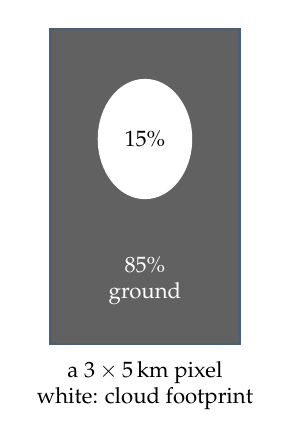
\begin{tikzpicture}[x=1mm,y=1mm]
 \fill[black!62](0,0)rectangle(24,40);
 % Cloud footprint in plan view: pi * 6 * 7.639437 = 144 mm^2,
 % exactly 15 percent (to rounding) of the 24 * 40 mm^2 pixel.
 \fill[white](12,26)ellipse(6 and 7.639437);
 \node[font=\footnotesize]at(12,26){15\%};
 \node[text=white,font=\footnotesize,align=center]at(12,8){85\%\\ground};
 \draw[pisablue,line width=.8pt](0,0)rectangle(24,40);
 \node[below,font=\footnotesize,align=center]at(12,-1){a $3\times5$\,km pixel\\white: cloud footprint};
\end{tikzpicture}
\column{.68\textwidth}
{\large\textcolor{sevrss}{\textbf{Image}}}\par\smallskip
The small cumulus raises reflectance from 10\% to 19\%.\par\bigskip
{\large\textcolor{feasible}{\textbf{Cloud mask}}}\quad one label for the whole pixel\par\smallskip
A small cumulus may not trigger a \textbf{``cloudy''} label.
\end{columns}
\vfill
\takeaway{Our thermal study targets small cumuli, which the standard mask can miss. We therefore want to use images, especially HRV.}
\speaker{\textbf{Why small cumuli matter.} A small cumulus may cover too little of a coarse SEVIRI pixel to trigger the standard cloud classification. A ``clear'' label therefore does not rule out a small cumulus. The classifier combines spectral tests, with no universal cloud-area threshold.\par\smallskip
\textbf{Illustrative mixed pixel.} The white ellipse occupies 15\% of the rectangle, with ground covering 85\%. These are illustrative area fractions. With ground reflectance 10\% and cloud reflectance 70\%, the average is $0.85\times10\%+0.15\times70\%=19\%$. This continuous signal gives no cloud position within the pixel.\par\smallskip
\textbf{Why HRV.} Bley and Deneke (2013) show that HRV can detect small convective clouds missed by the coarser standard mask. Its spatial and optical-thickness limits still prevent detection of every small cumulus. Conversely, many partly cloudy coarse pixels receive a cloudy label, which can overestimate cloud fraction.\par\smallskip
\textbf{Source.} Bley and Deneke (2013), Atmospheric Measurement Techniques, 6, 2713--2723, doi:10.5194/amt-6-2713-2013.
}
\end{frame}

\section{Limits}

\begin{frame}{Parallax: clouds appear north of where they are}
\vfill
\begin{columns}[c,onlytextwidth]
\column{.52\textwidth}
\centering
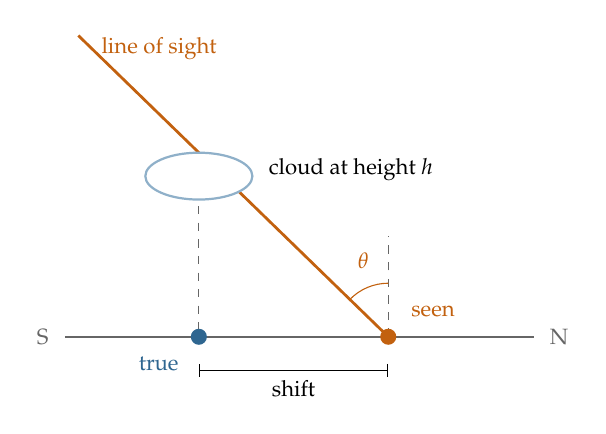
\begin{tikzpicture}[x=.85mm,y=.85mm,font=\footnotesize]
 \draw[muted,line width=.8pt](0,0)--(70,0);
 \draw[muted,dashed](20,22)--(20,0);
 \draw[mtg,line width=1pt](2,45)--(48.3,0);
 \fill[white,draw=sevfull,line width=.8pt](20,24)ellipse(8 and 3.5);
 \draw[muted,dashed](48.3,0)--(48.3,15);
 \draw[mtg](48.3,8)arc(90:135.8:8);\node[text=mtg]at(44.6,11.4){$\theta$};
 \fill[sevrss](20,0)circle(1.2);\fill[mtg](48.3,0)circle(1.2);
 \draw[|-|](20,-5)--node[below]{shift}(48.3,-5);
 \node[anchor=west]at(29,25){cloud at height $h$};
 \node[anchor=south west,text=mtg]at(4,40){line of sight};
 \node[anchor=north,text=sevrss]at(14,-1.5){true};
 \node[anchor=south,text=mtg]at(55,1.5){seen};
 \node[anchor=east,text=muted]at(-1,0){S};\node[anchor=west,text=muted]at(71,0){N};
\end{tikzpicture}
\column{.44\textwidth}
\large
\[\text{shift}=h\,\tan\theta\approx1.2\text{--}1.5\times h\]
{\small $\theta$: angle of the line of sight from vertical,\\ 50--57$^\circ$ over France}\par\medskip
\renewcommand{\arraystretch}{1.5}
\begin{tabular}{@{}lr@{}}
Cloud at 2.5\,km & 3--4\,km north\\
Cloud at 4\,km & 5--6\,km north\\
\end{tabular}
\end{columns}
\vfill
\takeaway{A cloud above a 10\,km cell can show up in the next cell to the north.}
\speaker{\textbf{Geometry.} Use a spherical Earth with $R=6371$ km and satellite radius $R_g=42164$ km. For latitude $\phi$, longitude $\lambda$ and satellite longitude $\lambda_s$ (9.5 E for RSS; 0 for MTG): $\cos c=\cos\phi\cos(\lambda-\lambda_s)$; $d^2=R^2+R_g^2-2RR_g\cos c$; $\sin\theta=(R_g/d)\sin c$. The horizontal shift is approximately $h\tan\theta$.\par\smallskip
\textbf{Examples.} At 45.3 N, 5.9 E, $c=45.4^\circ$, $d=37960$ km, $\theta=52.3^\circ$ and $\tan\theta=1.29$. Normandy (49 N, 0.45 W): $\theta\simeq57^\circ$, $\tan\theta\simeq1.54$. The finite satellite distance gives $\theta=c+\beta$, with $\beta$ about 7 degrees; Meteosat appears 33--40 degrees above the southern horizon. The shifts were also computed by tracing satellite--cloud rays to the WGS84 ellipsoid with pyproj.\par\smallskip
\textbf{Height assumption.} An elevated cloud appears mainly north of its true position when geolocation assumes sea level. The same effect applies to terrain. If cloud height were equated to the highest observed climb in each cell, the estimated shifts would be 3--3.7 km for plains/hills and 4--5 km for mountain cells. This equality is unvalidated: climb altitude need not represent cloud base or cloud top. Slide 11 explains the limitation and the proposed sensitivity check.}
\end{frame}

\begin{frame}{Parallax correction: small cumuli can lack height estimates}
\vfill
\begin{columns}[c,onlytextwidth]
\column{.38\textwidth}\centering
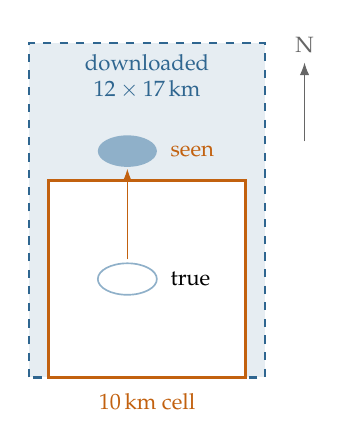
\begin{tikzpicture}[x=2.5mm,y=2.5mm,font=\footnotesize]
 \fill[sevrss!12](-1,0)rectangle(11,17);
 \draw[sevrss,dashed,line width=.9pt](-1,0)rectangle(11,17);
 \fill[white](0,0)rectangle(10,10);
 \draw[mtg,line width=1.2pt](0,0)rectangle(10,10);
 \node[text=mtg,anchor=north]at(5,-.3){10\,km cell};
 \node[text=sevrss,align=center]at(5,15.3){downloaded\\$12\times17$\,km};
 \fill[white,draw=sevfull,line width=.6pt](4,5)ellipse(1.5 and .8);
 \fill[sevfull](4,11.5)ellipse(1.5 and .8);
 \draw[-{Latex[length=1.6mm]},mtg](4,6)--(4,10.6);
 \node[anchor=west,text=mtg]at(5.7,11.5){seen};
 \node[anchor=west]at(5.7,5){true};
 \draw[-{Latex[length=1.6mm]},muted](13,12)--(13,16);\node[text=muted]at(13,16.9){N};
\end{tikzpicture}
\column{.58\textwidth}
\stepitem{1}{Satellite cloud-top height is the intended input for parallax correction}\medskip
\stepitem{2}{\textcolor{mtg}{\textbf{Small cumuli may only partly fill a pixel.}}\\Cloud and ground signals mix; MTG's height product excludes fractional clouds.}\medskip
\stepitem{3}{Climb heights are a possible fallback?}
\end{columns}
\vfill
\takeaway{The day's highest altitude reached in a climb need not mark cloud base and does not measure cloud top.}
\source{\href{https://user.eumetsat.int/catalogue/EO:EUM:DAT:0681}{EUMETSAT MTG cloud-top temperature and height}: fractional clouds excluded. \href{https://satpy.readthedocs.io/en/stable/api/satpy.modifiers.parallax.html}{Satpy}: correction uses a supplied height.}
\speaker{\textbf{Satellite-height limitation.} A reliable cloud-top height is the intended input. Small cumuli may only partly fill a pixel, mixing cloud and surface radiation. EUMETSAT's MTG Cloud Top Temperature and Height product (EO:EUM:DAT:0681) excludes fractional clouds because accurate height estimation is not possible. This is a product-specific limitation, not a claim that all small cumuli lack estimates.\par\smallskip
\textbf{Unvalidated fallback.} The day's highest climb may be below cloud base, unrelated to clouds, or from another time or location. Even a valid cloud-base proxy would not establish cloud-top height. Missing satellite estimates do not validate this replacement.\par\smallskip
\textbf{Proposed check.} Use reliable satellite heights where available. Otherwise compare candidate heights with independent, time-matched evidence and test a plausible range. Report the spread in corrected positions; $\delta d\simeq\tan\theta\,\delta h$. Sensitivity analysis does not itself validate the proxy.\par\smallskip
\textbf{Download.} Retain the original images and the proposed 12 by 17 km crop (7 km north, 1 km each side). Check that its margins cover the heights considered. Sources: EUMETSAT product description and Satpy documentation linked on the slide.}
\end{frame}

\section{Our study}

\begin{frame}{Our study: twelve 10 km windows}
\centering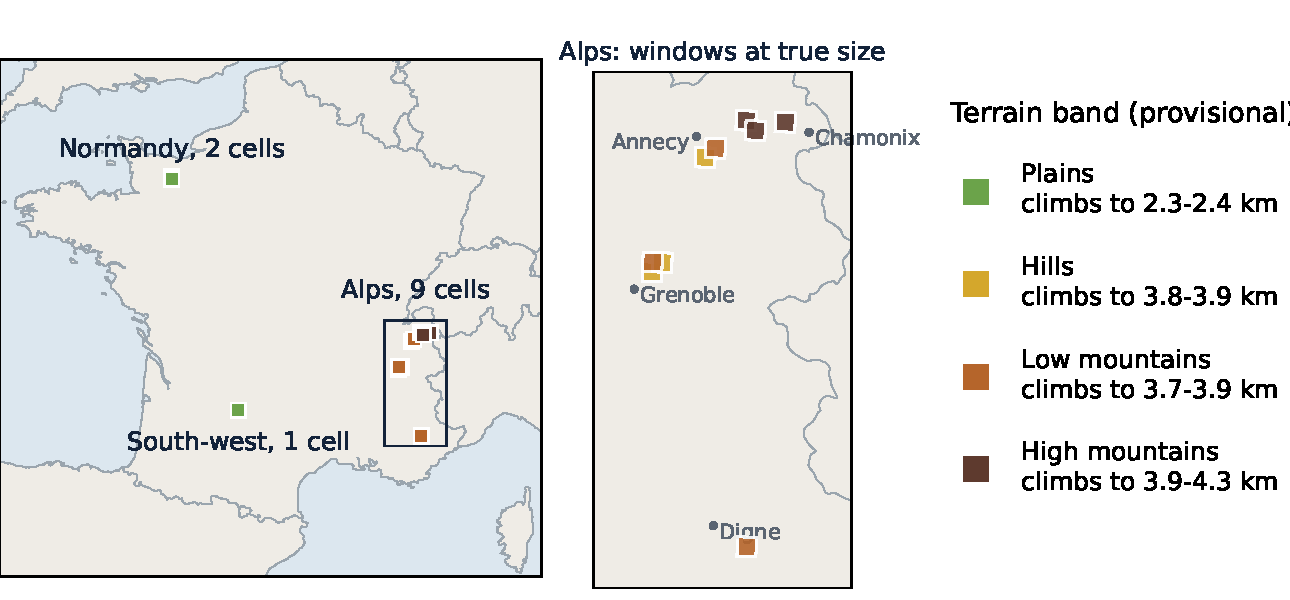
\includegraphics[width=\linewidth,height=50mm,keepaspectratio]{assets/cells-map.pdf}\par
\takeaway{Every 5\,min? 15min?, 2008--2026? 2008--2023?, 08:00--20:00 ?}
\source{Terrain band: highest IGN DEM elevation inside each 5\,km cell.}
\speaker{The three cells with the most Vilpellet climbs in each band of the highest IGN elevation inside the cell (below 300 m, 300--800, 800--1500, above 1500 m). One summit pixel is enough to lift a cell into a higher band, so the bands describe the highest relief in the cell. Cells (ix/iy, 5 km Lambert-93 lattice): plains 89/1375, 88/1376, 89/1373; hills 89/1374, 114/1275, 169/1388; low mountains 105/1242, 183/1292, 183/1300; high mountains 190/1306, 184/1293, 185/1294. The ranking skipped one cell that the French elevation model does not cover: 102/1221, at \`{A}ger in Catalonia. Each window is the 10 by 10 km Zoom-out view of Thermal planes, centred on the 5 km cell, plus 7 km to the north for parallax. Highest climb: the highest altitude any flight reached in the cell. Source: viewer store thermal-planes.sqlite3, ranking vilpellet-climb-runs-dem-max-top-v1.}
\end{frame}



\begin{frame}{What each dataset would show in a 10 km cell, over one hour}
\centering
\ifdefined\Speakernotes
 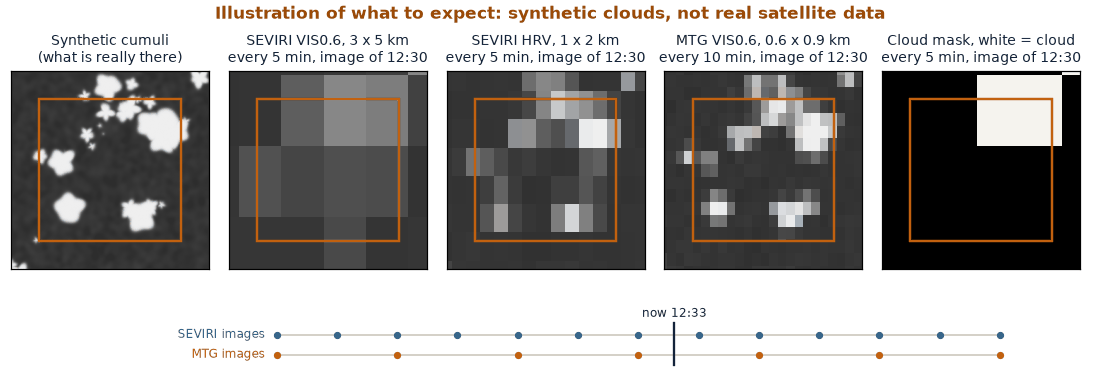
\includegraphics[width=\linewidth]{assets/expected/frames/frame-33.png}
\else
 \animategraphics[autoplay,loop,poster=first,width=\linewidth]{4}{assets/expected/frames/frame-}{00}{60}
\fi\par
\hfill{\footnotesize\href{run:assets/expected/expected-views.gif}{Open GIF}}
\takeaway{Illustration, not data. At $3\times5$\,km, SEVIRI is too coarse for our analyses; HRV shows the larger cumuli, MTG single clouds. Each panel changes only when its satellite takes an image.}
\speaker{The first panel is an invented field of fair-weather cumuli at 50 m resolution. The other image panels show pixel-averaged brightness from the latest simulated acquisition. The coarse cloud-mask panel uses an arbitrary 25\% cloud-area threshold for illustration. It implements neither the operational EUMETSAT classifier nor the Bley--Deneke HRV method. There is no universal cloud-area threshold in those methods. The 3 by 5 km channels cannot locate cumuli inside the cell. Infrared channels provide cloud-temperature information, while the 1.6 micrometre channel helps distinguish snow from cloud. Real images are blurrier and shifted by parallax; both effects are omitted here. This synthetic hour has one frame per minute. Cumuli form mostly over four fixed hot spots, live 15 to 35 minutes and drift east at 2 m/s. The dots mark simulated acquisitions every 5 minutes for SEVIRI and every 10 minutes for MTG. Between acquisitions, each panel stays frozen.}
\end{frame}



\begin{frame}{Three quarters of our flight-days fall in the cheap years}
\vfill\centering
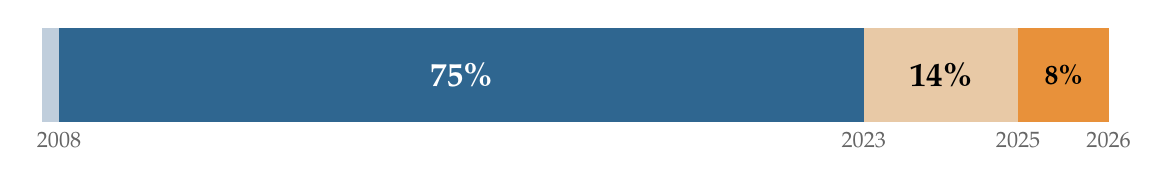
\begin{tikzpicture}[x=1mm,y=1mm]
 \fill[pisablight](0,0)rectangle(2.2,12);
 \fill[sevrss](2.2,0)rectangle(104.4,12);\node[text=white,font=\large\bfseries]at(53.3,6){75\%};
 \fill[gap](104.4,0)rectangle(124.0,12);\node[font=\large\bfseries]at(114.2,6){14\%};
 \fill[mtglight](124.0,0)rectangle(135.5,12);\node[font=\bfseries]at(129.8,6){8\%};
 \foreach \x/\y in {2.2/2008,104.4/2023,124.0/2025,135.5/2026}{\node[below,font=\footnotesize,text=muted]at(\x,0){\y};}
\end{tikzpicture}
\vfill
\begin{columns}[T,onlytextwidth]
\column{.32\textwidth}\textcolor{sevrss}{\textbf{2008--2022}}\par\small SEVIRI copy: cheap
\column{.32\textwidth}\textcolor{feasible}{\textbf{2023--2024}}\par\small SEVIRI files: expensive
\column{.32\textwidth}\textcolor{mtg}{\textbf{2025--2026}}\par\small MTG: feasible
\end{columns}
\vfill
\takeaway{SEVIRI runs to today; only its cheap copy stops in 2022.}
\speaker{Flight-days in the 12 cells: summer days times cells crossed, from the viewer table summer\_days, 30,850 in total; 2 percent fall before 2008, without 5-minute data. In 2023--2024 the SEVIRI images exist only as whole-Europe EUMETSAT files, 58 MB every 5 minutes. From late 2024, MTG offers sharper images every 10 minutes at a feasible cost.}
\end{frame}

\begin{frame}{Plan and space needed}
\vfill
\large\renewcommand{\arraystretch}{1.35}
\begin{tabularx}{\linewidth}{@{}rLrr@{}}\toprule
 & & Kept & Downloaded\\\midrule
1 & SEVIRI images 2008--2022, OCF copy & 5.4\,GB & 420\,GB\\
2 & SEVIRI cloud mask 2008--2026 & 0.16\,GB & 85\,GB\\
3 & MTG images 2024--2026, 3 strips & 1.1\,GB & 3.3\,TB\\
4 & Optional: SEVIRI cloud-top height & 0.13\,GB & 149\,GB\\\midrule
 & \textbf{Total} & \textbf{$\approx$\,7\,GB} & \textbf{$\approx$\,4.0\,TB}\\\bottomrule
\end{tabularx}
\vfill
\takeaway{Left out: SEVIRI images for 2023--2026, 11.6\,TB to download for 1.2\,GB kept.}
\speaker{Kept: 10 km windows plus the 7 km northern margin, 08:00--20:00 only. Downloaded: the files or blocks that hold the cells; about 3.7 days at 100 Mbit/s in total. Row 1 is measured on a pilot day (25 July 2020: 89 MB downloaded in 8.5 seconds, 1.1 MB kept; HRV and the 3 km visible channels match best at zero shift, correlation 0.998) and scaled to the days the archive holds. The other rows use catalogue file sizes. Also not planned: MTG all 16 channels (3.2 TB), MTG cloud products (2.2 TB). Each block is cropped in memory and dropped; parallax is not applied to the stored data. Rows 2--4 need a free EUMETSAT account.}
\end{frame}

\begin{frame}{Sources}
\footnotesize
\refitem{https://data.eumetsat.int}{EUMETSAT Data Store: product descriptions, counts and file sizes}{queried 6 Oct 2026}
\refitem{https://console.cloud.google.com/storage/browser/public-datasets-eumetsat-solar-forecasting/satellite/EUMETSAT/SEVIRI_RSS/v4}{Open Climate Fix SEVIRI rapid-scan Zarr, public bucket}{block sizes measured 6 Oct 2026}
\refitem{https://github.com/openclimatefix/Satip}{Open Climate Fix Satip: channel scaling constants}{satip/constants.py}
\refitem{https://www-cdn.eumetsat.int/files/2020-07/pdf_mtg_fci_l1_pug.pdf}{MTG FCI Level 1 Product User Guide}{40 strips per scan}
\refitem{https://www.businesswire.com/news/home/20241204214350/de}{Meteosat-12 declared operational}{4 Dec 2024}
\refitem{https://asdnews.com/news/aerospace/2026/08/27/arianespace-successfully-launches-weather-satellite-mtgi2-ariane-6s-first-mission-geostationary-orbit}{MTG-I2 launch}{27 Aug 2026}
\refitem{https://doi.org/10.5194/amt-6-2713-2013}{Bley and Deneke (2013), HRV cloud mask}{EUMETSAT mask and sub-pixel cumuli}
\refitem{https://doi.org/10.5194/amt-14-5107-2021}{Deneke et al. (2021), HRV implementation}{Sect. 3.5 and data availability}
\refitem{https://doi.org/10.5281/zenodo.4936573}{Deneke et al. (2021), public example data}{case studies, not our full archive}
\refitem{https://space.oscar.wmo.int/instruments/view/seviri}{WMO OSCAR: SEVIRI}{sampling and field of view}
\refitem{https://satpy.readthedocs.io/en/latest/api/satpy.modifiers.parallax.html}{satpy parallax correction}{needs cloud-top height}
\par\medskip

\speaker{Everything marked as measured was queried or downloaded on 6 October 2026.}
\end{frame}

\end{document}
